\chapter{Introduction}
\label{chap:intro}

\section{The Ubiquity of Synthetic and Screen Content}
Over the past decade, digital video transmission has undergone a profound structural shift. While traditional video workflows centered almost exclusively around photographic and cinematic video captured by physical optical sensors, a massive fraction of modern video bandwidth is now occupied by \textit{synthetic and computer-generated screen content}. This includes:
\begin{itemize}
    \item Remote desktop protocol (RDP) sessions and virtual desktop infrastructures (VDI) enabling hybrid work;
    \item High-definition screen recordings, software tutorials, and programming broadcasts;
    \item Digital slide presentations and collaborative whiteboard applications in enterprise and educational environments;
    \item Cloud gaming and interactive application streaming;
    \item Stylized 2D and cel-shaded digital animations.
\end{itemize}

Unlike natural video, screen content exhibits distinct structural properties. Natural video is characterized by continuous gradients, organic textures, sensor noise, and smooth camera motions. In contrast, screen content is characterized by large spatially homogeneous regions, razor-sharp single-pixel edges, high-contrast typography, and strict color palettes. Temporally, screen content frequently remains completely static over dozens or hundreds of frames, punctuated by localized updates (such as a blinking text cursor, scrolling viewport, or button hover state).

\section{Fundamental Limitations of Block-Based Hybrid Codecs}
Virtually all mainstream digital video coding standards developed over the past three decades---including ITU-T H.264 / MPEG-4 AVC~\cite{wiegand2003overview}, H.265 / HEVC~\cite{sullivan2012overview}, H.266 / VVC~\cite{bross2021overview}, and AOMedia AV1~\cite{chen2020overview}---share a common foundational architecture known as the \textit{hybrid block-based transform coding paradigm}.

Under this architecture:
\begin{enumerate}
    \item Frames are partitioned into square spatial blocks (macroblocks or Coding Tree Units ranging from $4\times 4$ to $128\times 128$ pixels).
    \item Temporal redundancy is exploited via block motion estimation and motion compensation, producing a spatial residual block.
    \item Spatial redundancy of the residual is compressed using 2D frequency transforms, predominantly the Discrete Cosine Transform (DCT) or Discrete Sine Transform (DST).
    \item Quantization of transform coefficients introduces loss, followed by context-adaptive entropy coding (CABAC or ANS).
    \item Color is typically downsampled to the $4:2:0$ chroma subsampling format to exploit human visual acuity limits.
\end{enumerate}

While this paradigm achieves exceptional compression efficiency on natural video, it encounters severe theoretical and practical bottlenecks when confronted with screen and UI content:
\begin{itemize}
    \item \textbf{High-Frequency Transform Ringing:} The DCT is optimal for signals modeled by first-order Gauss-Markov processes with smooth spatial correlations. At sharp step edges---such as black text on a white canvas---truncation of high-frequency DCT coefficients manifests as severe \textit{Gibbs ringing} and mosquito noise, degrading text legibility.
    \item \textbf{Chroma Bleeding from Subsampling:} $4:2:0$ chroma subsampling decimates color resolution by a factor of four. While unnoticeable in natural scenes, it causes catastrophic color fringing and illegibility on single-pixel colored text, code syntax highlighting, and UI icons.
    \item \textbf{Block Boundary Artifacts:} Independent block quantization produces visible discontinuities along block boundaries, breaking straight horizontal and vertical lines prevalent in user interfaces.
    \item \textbf{Motion Search Inefficiency for Micro-Updates:} When a tiny element (such as a 12-pixel cursor) updates in an otherwise static $1080\text{p}$ or $4\text{K}$ frame, block partitioning structures still incur significant header, split-flag, and motion vector overhead.
\end{itemize}

Although extensions such as HEVC Screen Content Coding (HEVC-SCC)~\cite{xu2015overview} introduced specialized tools (such as Intra Block Copy and Palette Mode), they add immense computational complexity and remain tethered to the underlying block-based framework.

\section{The Per-Pixel Temporal Function Hypothesis}
This thesis investigates an orthogonal question: \textit{What if video compression discarded spatial block transforms entirely, and instead operated directly on continuous 1D temporal trajectories of individual pixels?}

Consider a video sequence as a discrete four-dimensional tensor $V(t, y, x, c)$, where $t \in \{0, \dots, T-1\}$ denotes time, $(x, y)$ denotes spatial coordinates, and $c \in \{\text{R}, \text{G}, \text{B}\}$ denotes color channels. For a fixed pixel location $(x, y)$ and channel $c$, the temporal sequence:
\begin{equation}
    s(t) = V(t, y, x, c), \quad t \in \{0, 1, \dots, T-1\}
\end{equation}
forms a one-dimensional signal. On temporally coherent content, $s(t)$ is not an arbitrary sequence of independent values; rather, it is often piece-wise constant (static UI), piece-wise linear (gradual luminance fades, smooth scroll transitions), or smoothly varying.

\begin{figure}[t]
    \centering
    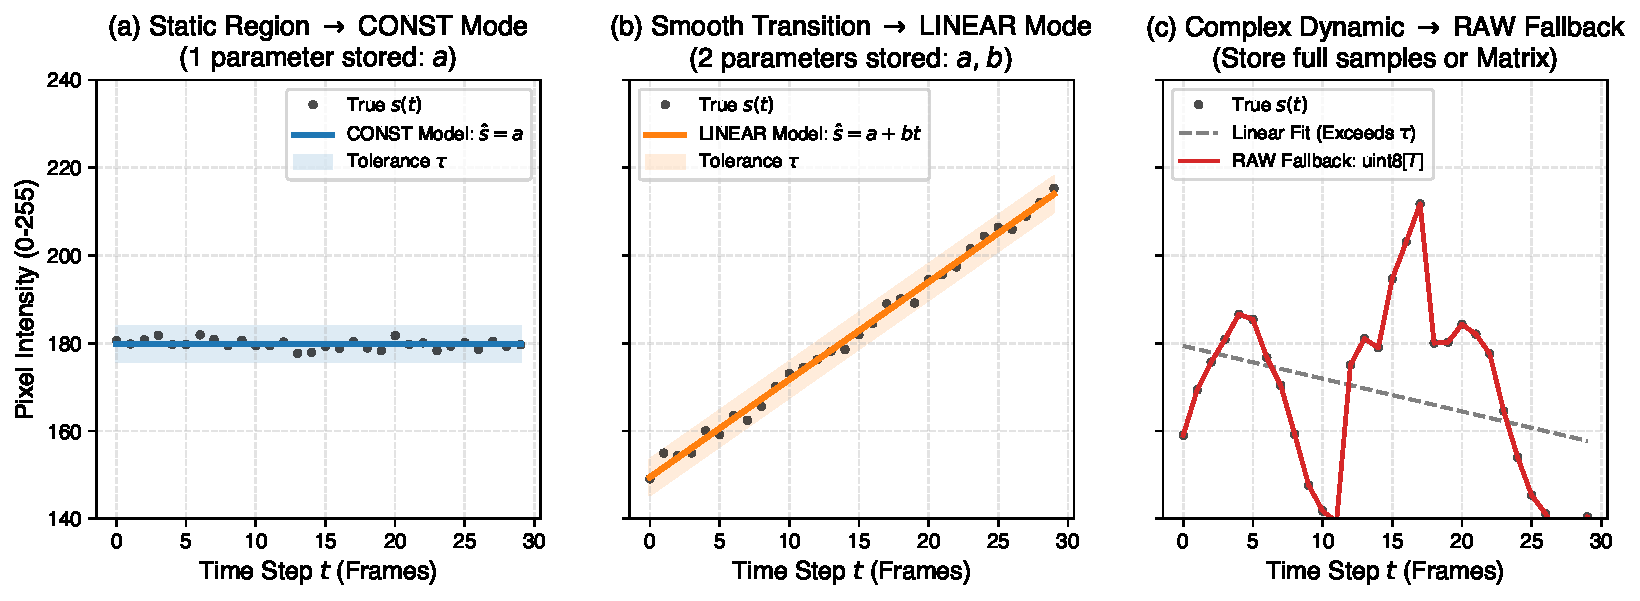
\includegraphics[width=\linewidth]{figures/temporal_fitting_concept.pdf}
    \caption{Conceptual overview of TimeFlowCodec per-pixel temporal modeling. (a) Static UI regions are captured with a single constant parameter $a$. (b) Linear shifts and fades are modeled with parameters $(a, b)$. (c) Abrupt or complex transitions fall back to quantized raw sample arrays.}
    \label{fig:temporal_concept}
\end{figure}

The \textbf{TimeFlowCodec (TFC)} hypothesis posits that:
\begin{quote}
    \textit{Modeling temporal pixel trajectories using low-order parametric functions yields superior high-frequency spatial edge preservation, zero block boundary artifacts, native full-resolution RGB fidelity, and deterministic $\mathcal{O}(T)$ encoding and decoding complexity for screen and synthetic video.}
\end{quote}

Figure~\ref{fig:temporal_concept} illustrates this principle. By classifying each pixel's trajectory into \textsc{Constant}, \textsc{Linear}, or fallback modes based on a variance-normalized error ratio $\tau$, the encoder transmits only 1 or 2 scalar parameters per pixel over an entire temporal window, compressing the signal along the time dimension without altering spatial high-frequency edges.

\section{Key Research Contributions}
The primary contributions of this thesis are as follows:
\begin{enumerate}
    \item \textbf{Mathematical Formalization of Temporal Regression Coding:} We formulate closed-form Ordinary Least Squares solutions for constant and linear temporal models that stream in $\mathcal{O}(T)$ time and $\mathcal{O}(1)$ space per pixel, accompanied by an adaptive decision metric $\tau$ normalized by baseline signal variance.
    \item \textbf{The .tfc Bitstream and v5 Streaming Container:} We design and implement the .tfc container specification, evolving from initial monolithic containers to the v5 bounded-chunk streaming architecture that supports arbitrary video duration under a fixed memory ceiling, rational frame rate timing, and multiplexed audio streams.
    \item \textbf{Systems Engineering of a Bounded-Memory Codec:} We implement a production-ready Python/C-accelerated codec with disk memory-mapping fallbacks, cooperative worker lifecycle cancellation, vectorized SIMD array decoding, and an interactive desktop player.
    \item \textbf{Comprehensive Empirical Evaluation:} We benchmark TimeFlowCodec against industry standards (H.264/AVC, H.265/HEVC, and AOMedia AV1) across four distinct visual domains: Screen/UI captures, slide presentations, stylized animations, and natural video, reporting objective metrics (RGB PSNR, windowed SSIM, encoding/decoding throughput, and memory footprint).
    \item \textbf{Information-Theoretic Boundary Analysis:} We rigorously characterize the operational limits and failure modes of temporal function coding under high-entropy sensor noise and unstructured natural motion, providing an analytical framework for hybrid temporal-spatial architectures.
\end{enumerate}

\section{Thesis Organization}
The remainder of this thesis is structured as follows:
\begin{itemize}
    \item \textbf{Chapter~\ref{chap:related_work}} reviews foundational video coding standards, screen content coding extensions, 1D transforms, and neural video compression.
    \item \textbf{Chapter~\ref{chap:theory}} derives the mathematical foundation of per-pixel temporal regression, error-ratio mode decisions, and rank-1 matrix approximations.
    \item \textbf{Chapter~\ref{chap:bitstream}} specifies the .tfc bitstream format across container versions v1 through v5.
    \item \textbf{Chapter~\ref{chap:implementation}} details the software architecture, memory bounding mechanisms, vectorized decoder, and desktop inspection engine.
    \item \textbf{Chapter~\ref{chap:evaluation}} presents quantitative rate-distortion curves, perceptual quality comparisons, and throughput benchmarks.
    \item \textbf{Chapter~\ref{chap:discussion}} analyzes algorithmic ablations, parameter sensitivities ($\tau$, tiling), and failure modes.
    \item \textbf{Chapter~\ref{chap:future_work}} outlines future research directions, including higher-order orthogonal polynomials, spline interpolation, and GPU compute kernels.
    \item \textbf{Chapter~\ref{chap:conclusion}} concludes with a summary of findings and the broader implications of temporal function video coding.
\end{itemize}
